A continuación, un diagrama de secuencia que representa la ejecución de un movimiento ofensivo, en este caso un pase exitoso.

\begin{landscape}

  \begin{figure}[h!]
   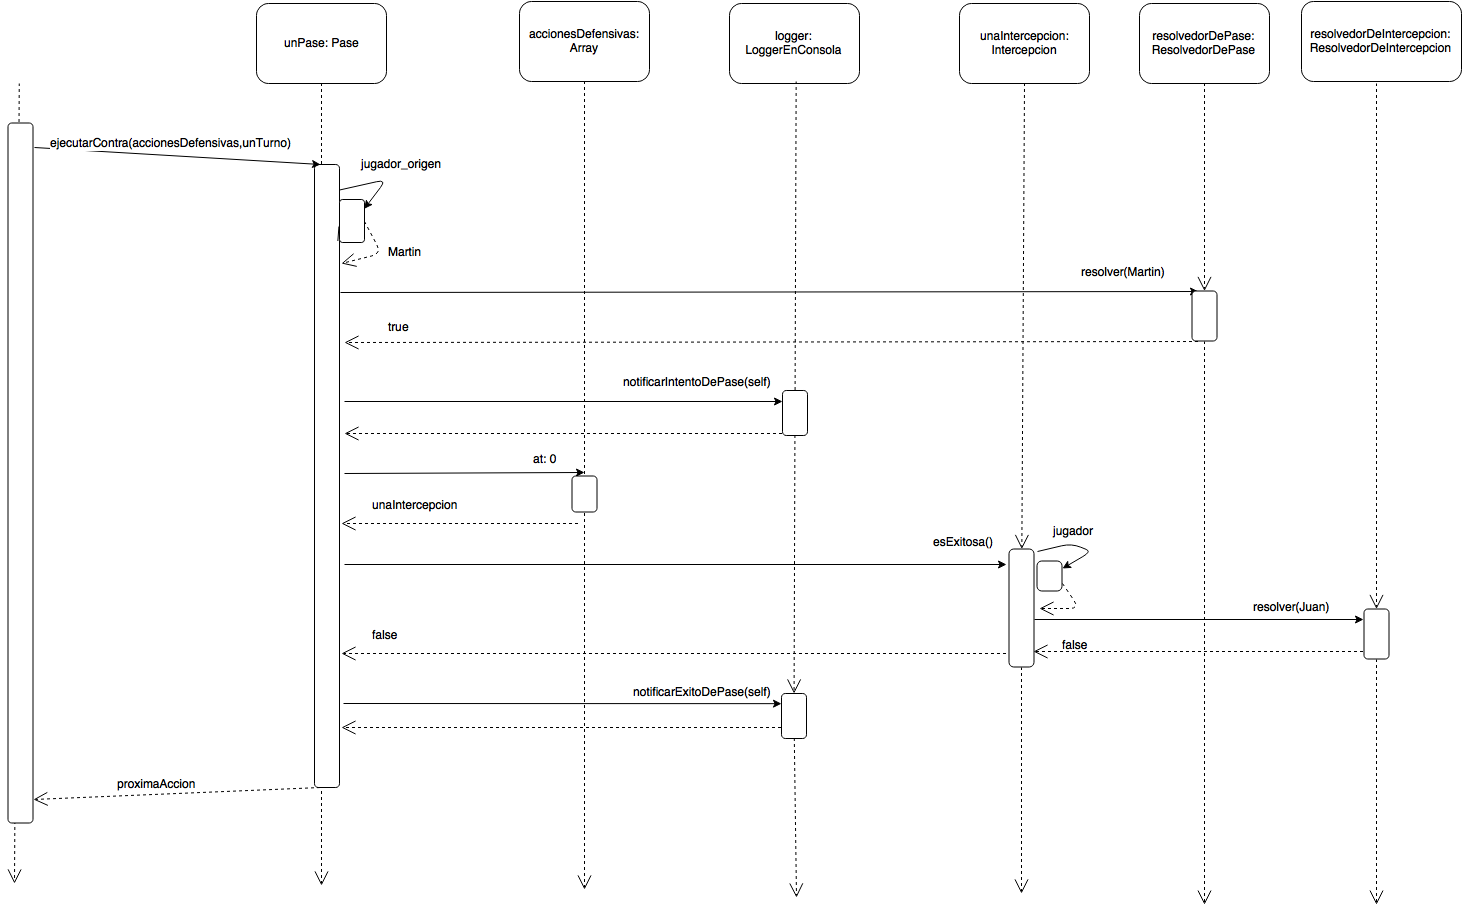
\includegraphics[scale=0.35]{imagenes/pase-exitoso.png}
   \caption{Un pase exitoso. Aclaración: se asume que el array de jugadas defensivas está compuesto por un único elemento para simplificar el diagrama.}
  \end{figure}

\end{landscape}

Como podemos observar en este diagrama de secuencia, el funcionamiento de un pase se encuentra fuertemente relacionado con una acción defensiva.
Un pase no va a tener éxito si una intercepción se lo impide. Este comportamiento se puede extender a cualquier movimiento ofensivo del juego.
Es por este motivo que tomamos la decisión de encapuslar este comportamiento de acción-reacción dentro de cada movimiento ofensivo
de manera que una acción ofensiva tenga éxito solo si la acción ofensiva tiene éxito y además la defensiva falla. 

Para los movimientos defensivos tenemos un comportamiento distinto. Ya no existen acciones que las contrarresten, no hay reaccion frente a ellas.
Si son exitosas, se ejecutan desde el contexto de un movimiento ofensivo. 

Para modelar el comportamiento descripto realizamos el siguiente diseño:

\begin{figure}[h!]
  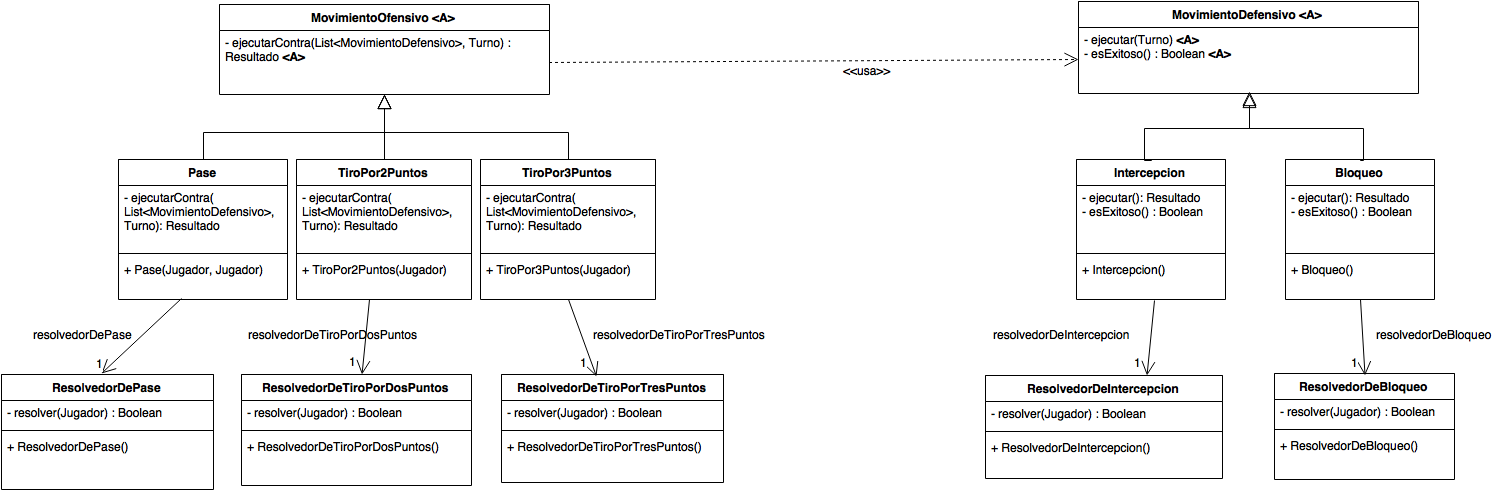
\includegraphics[scale=0.25]{imagenes/diagrama-clases-movimiento.png}
  \caption{Diagrama de clases para los movimientos ofensivos y defensivos}
\end{figure}

Para modelar el comportamiento común entre los movimientos ofensivos creamos una clase abstracta MovimientoOfensivo que sabe responder al mensaje ``ejecutarContra(unaAccionDefensiva)''. En el caso de los movimientos defensivos creamos una clase absracta MovimientoDefensivo que sabe responder a ``ejecutar()'' y ``esExitoso()''. 
